
%%%%%%%%%%%%%%%%%%%%%%%%%%%%%%%%%%%%%%%%%%%%%%%%%%%%%%%%%%%%%%%%%%%%%%%%%%%%%%%
%
%  EGSnrc manual for GUIs
%  Copyright (C) 2021 National Research Council Canada
%
%  This file is part of EGSnrc.
%
%  EGSnrc is free software: you can redistribute it and/or modify it under
%  the terms of the GNU Affero General Public License as published by the
%  Free Software Foundation, either version 3 of the License, or (at your
%  option) any later version.
%
%  EGSnrc is distributed in the hope that it will be useful, but WITHOUT ANY
%  WARRANTY; without even the implied warranty of MERCHANTABILITY or FITNESS
%  FOR A PARTICULAR PURPOSE.  See the GNU Affero General Public License for
%  more details.
%
%  You should have received a copy of the GNU Affero General Public License
%  along with EGSnrc. If not, see <http://www.gnu.org/licenses/>.
%
%%%%%%%%%%%%%%%%%%%%%%%%%%%%%%%%%%%%%%%%%%%%%%%%%%%%%%%%%%%%%%%%%%%%%%%%%%%%%%%
%
%  Authors:         Joanne Treurniet
%                   Blake Walters
%                   Iwan Kawrakow
%                   Dave Rogers
%
%  Contributors:
%
%%%%%%%%%%%%%%%%%%%%%%%%%%%%%%%%%%%%%%%%%%%%%%%%%%%%%%%%%%%%%%%%%%%%%%%%%%%%%%%


\documentclass[12pt,twoside]{article}
%\documentclass[12pt]{article}
%\usepackage{overcite}

\setlength{\textwidth}{16.51cm}
%\setlength{\textheight}{23.2cm}
\setlength{\textheight}{23.5cm}
\setlength{\oddsidemargin}{0.0in}
\setlength{\evensidemargin}{0.0in}
\setlength{\topmargin}{-1.5cm}
\setlength{\parindent}{1.5em}
\setlength{\topsep}{0ex}
\setlength{\itemsep}{0ex}

\newcommand{\Co}{$^{60}$Co}
\newcommand{\parsp}{~\hspace*{1.5em}}
\setlength{\parskip}{0.1in}
\setlength{\baselineskip}{1.0cm}
\newcommand{\head}[1]{\begin{center}\begin{Large}{\bf #1}
                                              \end{Large}\end{center}}
\newcommand{\cen}[1]{\begin{center} #1 \end{center}                   }
\newcommand{\cm}{component module}
\newcommand{\CM}{Component module}
\newcommand{\etal}{{\em et.al.}}
\newcommand{\ie}{{\em i.e.}}
\newcommand{\etc}{{\em etc.}}
\newcommand{\viz}{{\em viz.}}
\newcommand{\eg}{{\em eg.}}

\renewcommand{\refname}{}

\usepackage{epsf}

\usepackage{graphicx}
\usepackage{fancyhdr}
\renewcommand{\footrulewidth}{0.4pt}
\renewcommand{\headrulewidth}{0.4pt}

\lhead[{\sffamily \thepage}]{{\sffamily BEAMnrc, DOSXYZnrc and BEAMDP GUI User's Manual}}
\rhead[{\sffamily NRCC Report PIRS-0623(rev C)}]{{\sffamily ~\thepage}}
\rfoot[{\sffamily {\rightmark}}]{{\sffamily {\rightmark}}}
\lfoot[{\sffamily {\leftmark}}]{{\small Last edited $Date: 2013/03/29 15:20:27 $
}}
\cfoot{}

\usepackage{hyperref}
\hypersetup{colorlinks=true, citecolor=blue, linkcolor=blue, filecolor=blue, urlcolor=blue}
\urlstyle{same}

\usepackage{html}
\begin{latexonly}
\typeout{***Have turned off overfull and underfull messages****}
\tolerance=10000        %suppress Overfull only
\hbadness=10000         %suppress Overfull and Underfull for text (horizontal)
\vbadness=10000         %suppress Overfull and Underfull for vertical
			%"boxes"

\end{latexonly}


\makeindex
\begin{document}

\begin{htmlonly}
For information about the authors and/or institutions involved with this
work, use the links provided in the author list.\\
\begin{rawhtml}
<br><br>
\end{rawhtml}
\begin{rawhtml}
<br><br>
\end{rawhtml}
\begin{rawhtml}
<br><br>
\end{rawhtml}

Use the Up button to get back to this page from within the document.
\begin{rawhtml}
<BR> <HR> <P>
\end{rawhtml}
\copyright Copyright 2021, National Research Council of Canada, Ottawa
\begin{rawhtml}
<BR> <HR> <P>
\end{rawhtml}
\end{htmlonly}

\pagestyle{empty}

\title{BEAMnrc, DOSXYZnrc and BEAMDP GUI User's Manual}
\begin{center}
{\sffamily \bfseries \Huge BEAMnrc, DOSXYZnrc and BEAMDP GUI User's Manual \vspace{5mm}\\}
\begin{large}
J. R. Treurniet, B. R. Walters, I. Kawrakow and D. W. O. Rogers\\
\end{large}
Ionizing Radiation Standards\\
National Research Council of Canada\\Ottawa, K1A OR6\\

Printed: \today  \\
\hfill NRCC Report {\sf PIRS-0623(rev C)}\\

\end{center}

\vskip 0.8in

\begin{figure}[htbp]
\begin{center}
\htmlimage{scale=1.6}
\leavevmode
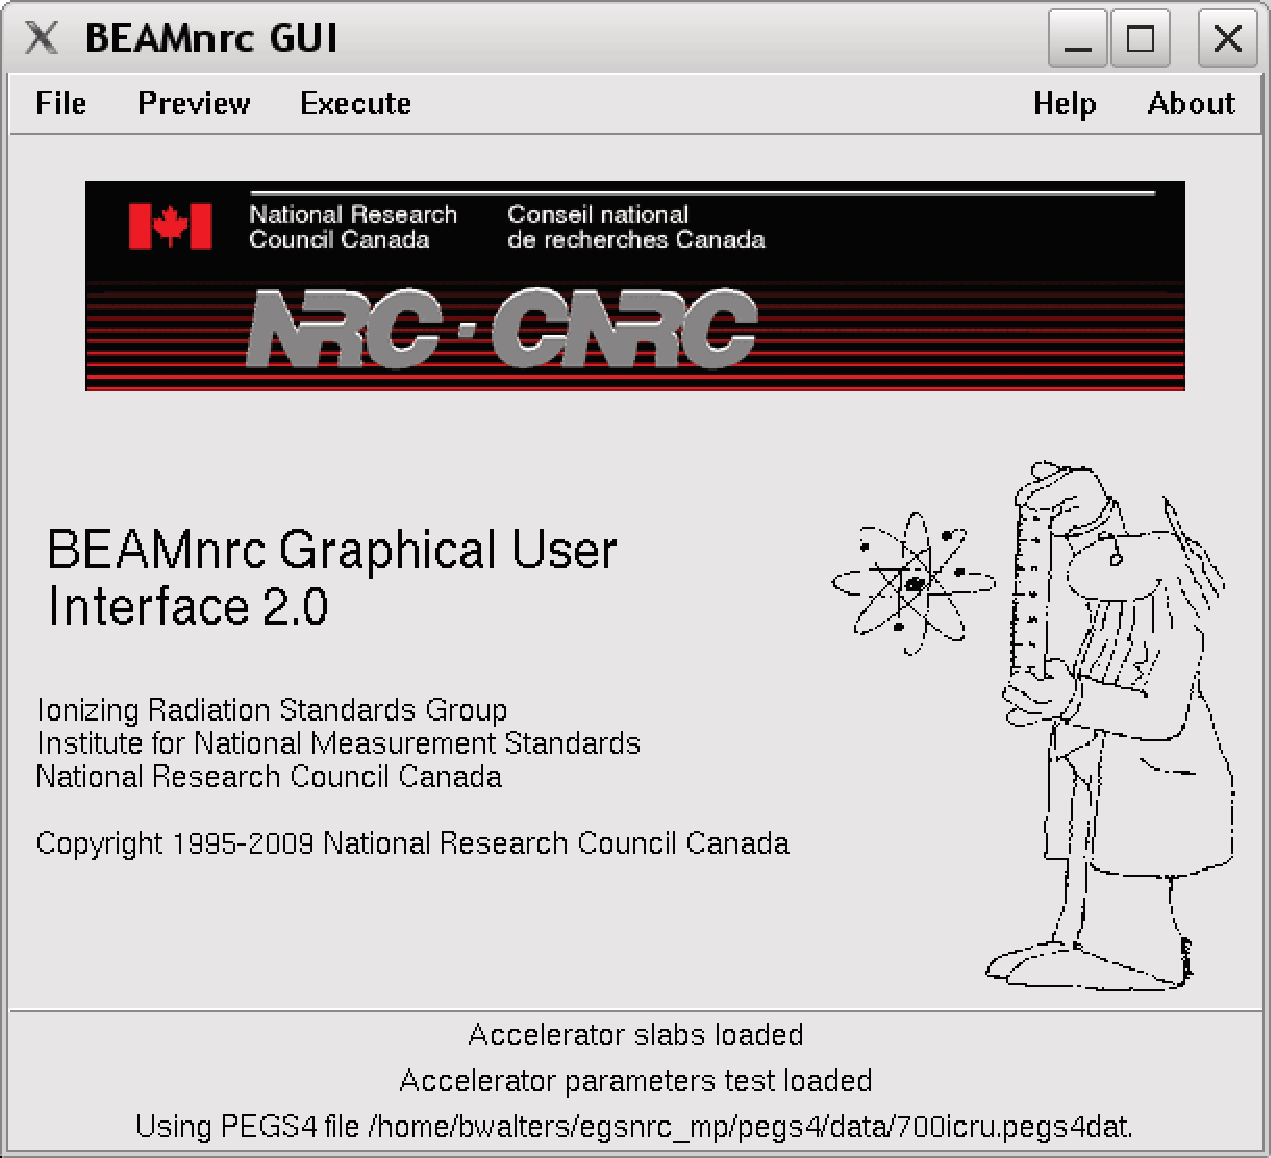
\includegraphics[width=14cm]{figures/gui_main_window}

The main window of the BEAMnrc GUI.
\end{center}
\end{figure}

%\maketitle

\vfill
\begin{center}
\copyright NRC Canada, 2021
\end{center}

\pagenumbering{arabic}
\setlength{\baselineskip}{0.5cm}

\newpage

\begin{center}
\begin{Large}
{\bf Abstract}
\end{Large}
\end{center}
The BEAMnrc GUI and the DOSXYZnrc GUI were created
for the generation of input files for the BEAMnrc and DOSXYZnrc codes.
They are equipped to compile and run BEAMnrc and DOSXYZnrc through the
interface.  The
BEAMDP GUI is a graphical front-end for the BEAMDP code.

This document reports how to get hold of and install the GUIs, and
briefly describes their capabilities.

%\vspace*{3cm}\\

\tableofcontents

\setlength{\baselineskip}{0.5cm}

\newpage

%\pagestyle{myheadings}

\section{Why YOU Need These GUIs!}

The BEAMnrc and DOSXYZnrc codes are large EGSnrc user-codes for simulating
radiotherapy units and doing CT based dose calculations, respectively
\cite{Ro95,WR04a,Ro04a}.  BEAMDP is a data processing tool for
use after BEAMnrc has been run\cite{MR04a,MR04b}.

For large and/or complicated accelerators, the input required for BEAMnrc can lead
to files which are large and confusing to the user.  Similarly the
inputs for DOSXYZnrc can be complex, especially for beams coming from
arbitrary directions.  The BEAMnrc and DOSXYZnrc GUIs were
created to aid the user in both creating and editing these files by
providing a label and a text box or option menu for each parameter, with
a detailed explanation available in a help window.  Much of the content
of the User's manuals \cite{WR04a,Ro04a} is actually available within
the GUIs, although the User's manuals represent the final authority.
An added benefit in the BEAMnrc GUI is
the preview option for each CM, wherein you may look at a graphical
representation of the CM that you have defined, a preview of the entire
accelerator, so that you may see the relative positioning of the CMs,
and a print/export option.

When the accelerator components and input parameters have been defined,
the GUIs write the files required to run the BEAMnrc or DOSXYZnrc code.

The interface to BEAMDP writes an input file based on the selections made and
runs BEAMDP with it.

\section{Getting and Installing the GUIs}

\subsection{Tcl/Tk}

All of the GUIs use {\tt Tcl/Tk} and {\tt wish}, a freeware package.
The GUIs were developed using {\tt Tcl} version 7.5, {\tt Tk} version
4.1 and {\tt wish} 4.1 or {\tt wishx}.  You
can obtain version 8.4 of {\tt Tcl/Tk} at
\htmladdnormallink{{\tt http://www.activestate.com/Products/ActiveTcl}}
{http://www.activestate.com/Products/ActiveTcl}.
Once you have installed {\tt Tcl/Tk} you must ensure that the directory
{\tt /(directory where Tcl/Tk was installed)/bin} is included in your
{\tt PATH} environment variable.

Note that most Linux distributions already include {\tt Tcl/Tk}, so there
is no need to download it (unless it's a version of {\tt Tcl/Tk}
that does not work with the GUIs).

Note that the makers of {\tt Tcl/Tk} have made no promises of backwards
compatibility.  We therefore cannot yet guarantee that these GUIs will
work for all versions of {\tt Tcl/Tk}, although we strive to do so in
the near future.  Version 8.4 appears to work satisfactorily with the
current versions of the GUIs.

\subsection{Installing the GUIs}

The GUIs are installed as part of the standard OMEGA/BEAM installation.
See the BEAMnrc Manual\cite{Ro04a} for complete instructions on how to
install the OMEGA/BEAM codes.

\section{The BEAMnrc GUI}

To run the BEAMnrc GUI from a Linux/Unix window, type {\tt beamnrc\_gui} at
the prompt.  Note that you must have sourced the Unix script
{\tt egsnrc\_cshrc\_additions}\\(or {\tt egsnrc\_bashrc\_additions}) in
your {\tt .cshrc} (or {\tt .bashrc}) file.  See the BEAMnrc Manual\cite{Ro04a}
for more information about these scripts.

To run the GUI in a Windows environment, either double click on
the GUI icon or use Windows Explorer to go into directory
{\tt \$OMEGA\_HOME/progs/gui/beamnrc} and double click on
{\tt beamnrc\_gui}.

The GUI generates two input files which are required by BEAMnrc.  The first is a
file with extension {\tt .module}, which contains the component modules
included in the accelerator and their identifying names.  These are
stored in the {\tt \$EGS\_HOME/beamnrc/spec\_modules} directory.  The
second file created has an extension {\tt .egsinp} and contains all of the
simulation parameters, and is usually stored in a directory
corresponding to its module filename, \ie~{\tt \$EGS\_HOME/BEAM\_}$<${\em
modulename}$>$.

\subsection{Setting the GUI defaults}

The BEAMnrc GUI loads a resource file when it starts, defining
colours and fonts for the application.  This file is called {\tt
.gui\_defaults} and is first searched for in your home directory, then in
the directory where the GUI code is stored if not found.  To change the
settings, copy the file from {\tt \$OMEGA\_HOME/progs/gui/beamnrc} to {\tt
\$HOME} and edit it to reflect your preferences.


\subsection{Specifying an accelerator}

The first step in using the GUI is to load an accelerator.  If you wish
to load a previously defined accelerator, select
the {\sf Load a previous accelerator} option from the main window {\sf File}
menu (shown on the front of this manual).  A browser will allow you to select
the file you wish to load from the {\tt \$EGS\_HOME/beamnrc/spec\_modules}
directory closest to the directory in which the GUI was started.
Otherwise, select the {\sf Specify a new
accelerator} option.  A window will appear which allows you to select
the CMs you would like to add to the accelerator, shown on the left of
figure~\ref{add_cm}.
Double-clicking a CM name on the list, or clicking once to select then
clicking the ``$>>$'' button, will insert
the CM name into the text box.  Enter an identifier name (maximum of 8
characters) then click {\sf Add} to add the CM to the accelerator.
The window on the right of figure~\ref{add_cm} shows the window which holds the
selected CMs.

\begin{latexonly}
\begin{figure}[htbp]
\begin{center}
\begin{minipage}[t]{9cm}
    \leavevmode
    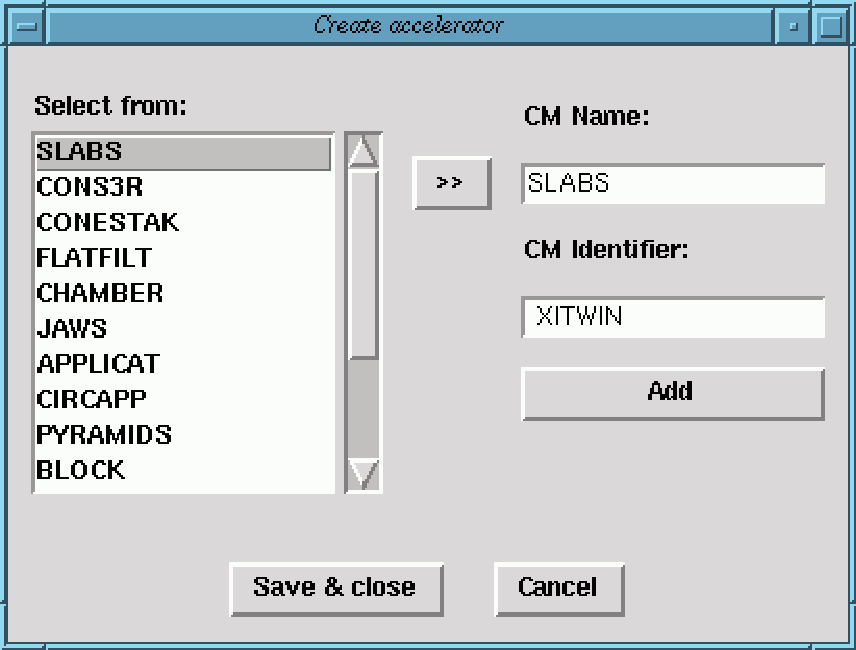
\includegraphics[width=8.5cm]{figures/add_cm}
\end{minipage}
\hfill
\begin{minipage}[t]{6cm}
    \leavevmode
    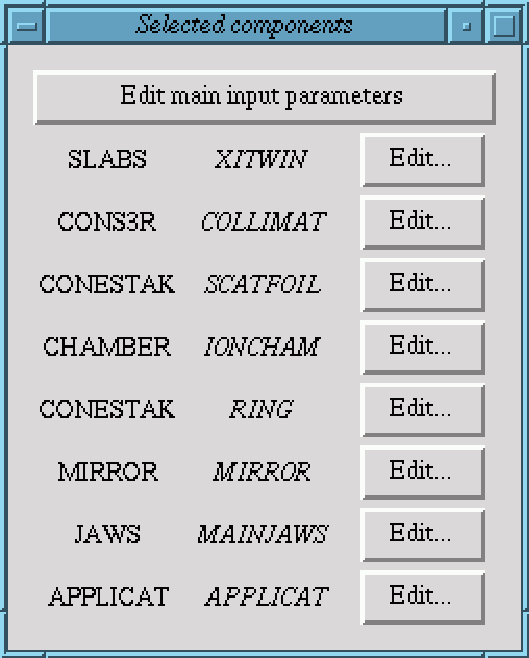
\includegraphics[width=5.5cm]{figures/cm_selected}
\end{minipage}
\end{center}
\caption{The windows for specifying a new accelerator (left) and for
displaying the selected CMs in the accelerator (right).\label{add_cm}}
\end{figure}
\end{latexonly}
\begin{htmlonly}
\begin{figure}[htbp]
\begin{center}
\htmlimage{scale=1.0}
    \leavevmode
    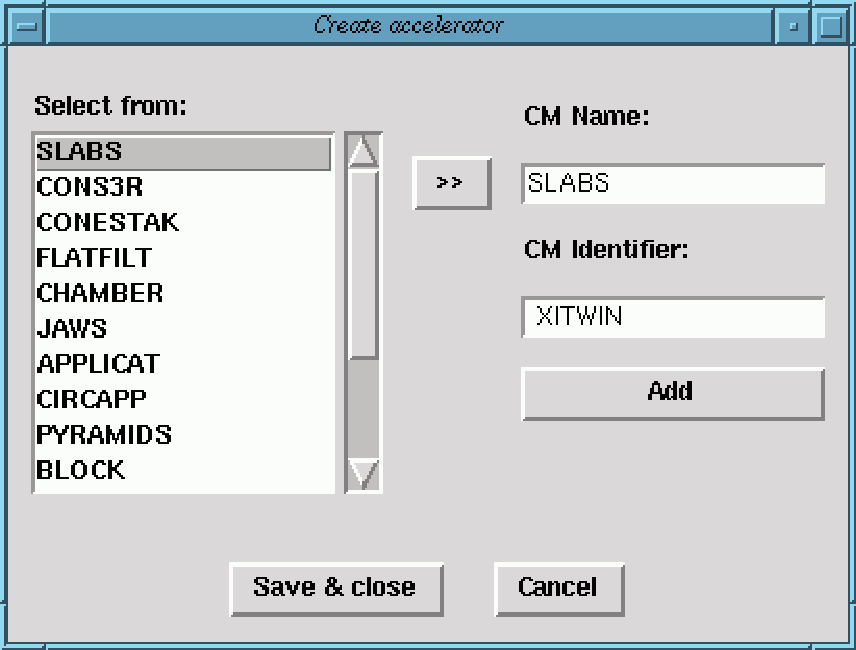
\includegraphics[width=15cm]{figures/add_cm}
\end{center}
\caption{The window for specifying a new accelerator.\label{add_cm}}
\end{figure}
\begin{figure}[htbp]
\begin{center}
\htmlimage{scale=1.0}
    \leavevmode
    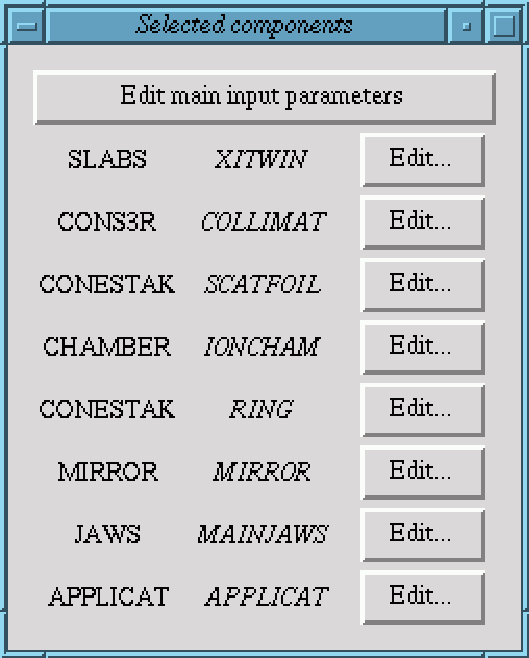
\includegraphics[width=10cm]{figures/cm_selected}
\end{center}
\caption{The window displaying the selected CMs in the accelerator.}
\end{figure}
\end{htmlonly}

When the accelerator has been completely specified, it must
be saved before continuing.  You don't have to enter the extension of
the filename; the GUI will do that for you.

\subsection{Loading PEGS4 cross-sectional data}

After the accelerator has been loaded or defined, you will be asked to
enter the name of the PEGS4 cross-sectional data file that you wish to
use.  This is so that the GUI can properly assign your options for
materials.  The full pathname of the file must be entered in the space
provided, so it is more efficient to simply browse directories.

If you have a PEGS4 file in both your user's {\tt \$EGS\_HOME/pegs4/data}
directory
and in the {\tt \$HEN\_HOUSE/pegs4/data} area, you must select the
one in your user's area.  This is
enforced because BEAMnrc first searches your user's {\tt \$EGS\_HOME/pegs4/data}
directory for the cross-sectional data file.

If at any time you wish to change the PEGS4 data file, you can select
the {\sf Change PEGS4 file} option on the main {\sf File} menu.  Note that you
will have to change the materials you have selected to correspond to the
new names.

\subsection{Defining simulation parameters}

After loading or specifying an accelerator, you are ready to define the
simulation parameters.  If
you have an input file already made, select {\sf Load a previous input
file} on the main window {\sf File} menu.  A browser will allow you to select
the file; it will search your directory tree for the directory
corresponding to the module loaded, \ie~{\tt BEAM\_}$<${\em
modulename}$>$, and if found, the browser will start
there.  Otherwise it will start in the directory in which the GUI was
started.  To change directories, double-click on the directory name.  To
select a file, single-click on the filename.

To edit the main simulation parameters, select the {\sf Edit main
parameters} button on the selected CMs window.
Each parameter on this window should be filled in.  You will be prompted
for additional related parameters.


The file {\tt \$OMEGA\_HOME/beamnrc/beamnrc\_user\_macros.mortran} contains
macros which define the default maximum and minimum values for some of
the main simulation parameters, as
well as the default maximum number of CMs allowed.  You will have to
edit this file (and recompile BEAMnrc) to change the values of these
parameters.

\subsubsection{EGSnrc input parameters}
\label{egsnrcinputsect}
Within the ``Main Inputs" window, there is a {\sf Edit EGSnrc Parameters}
button.  If you click on this, then a window opens which allows you to
adjust the EGSnrc input parameters (see Figure~\ref{egsnrcwindow}).
If you are working from an EGS4/BEAM input file or if you are starting
from scratch, then you will find that these EGSnrc inputs are set
to their default values (as they are in Figure~\ref{egsnrcwindow}).
The defaults are adequate for most accelerator simulations, however, you
may want to change parameters to take better advantage of EGSnrc's
improved physics, especially in low-energy applications.  When you save
the input file from the GUI, the EGSnrc input parameters are automatically
appended to the end of the {\tt .egsinp} file in a specific, text-based
format.  See the BEAMnrc manual for a more detailed description of the
EGSnrc inputs, their default values, and the input format.

\begin{figure}[htb]
\begin{center}
\htmlimage{scale=2.0}
\leavevmode
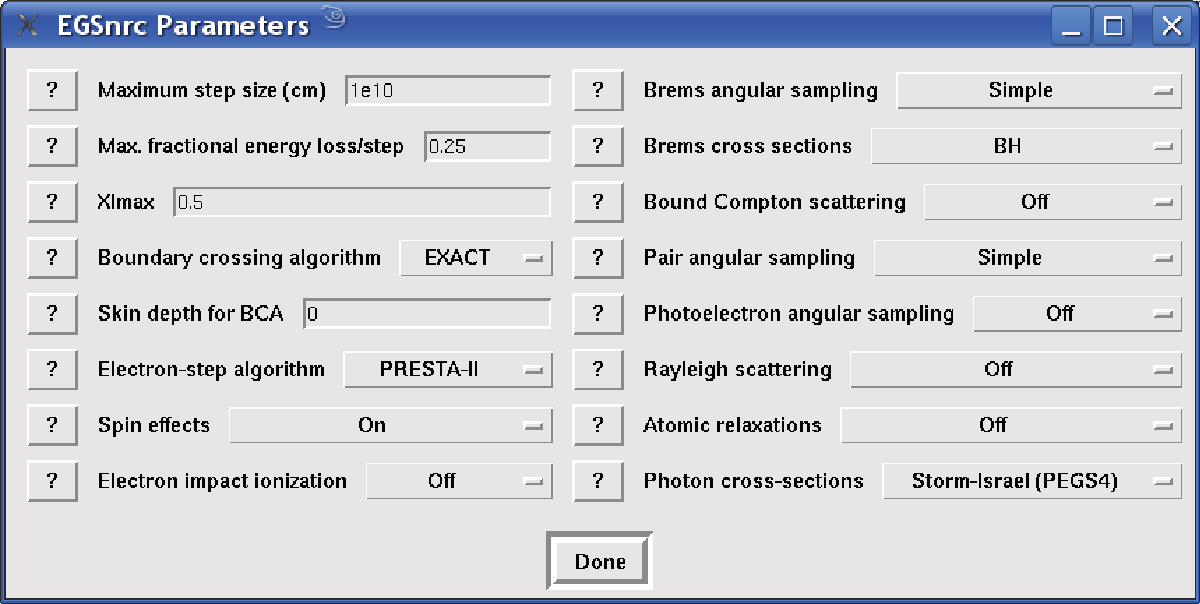
\includegraphics[width=14cm]{figures/egsnrc_inputs}
\end{center}
\caption{The EGSnrc input window with showing default values.}
\label{egsnrcwindow}
\end{figure}

\subsection{The fast track}

In the case where you have already made the module and input files you can start with the {\sf Load a
previous input file} option on the main window {\sf File} menu.  The browser
will start in the directory in which the GUI was started.  When you
select an input file, the GUI will search for the module filename which
corresponds to the input file selected and load it first, \ie~{\tt
BEAM\_}$<${\em modulename}$>$/$<${\em inputfile}$>$ should have it's
accelerator defined in {\em modulename}{\tt .module}.

Alternatively, if the accelerator has already been compiled and the input file exists
in the {\tt \$EGS\_HOME/BEAM\_accelname} directory, you can specify the input file
(and accompanying PEGS4 data) as command line arguments.  Within the
{\tt \$EGS\_HOME/BEAM\_accelname} directory type:
\begin{verbatim}
beam_gui inputfilename [pegsfilename]
\end{verbatim}
The {\tt .egsinp} and {\tt .pegs4dat} extensions on the input file and PEGS4 data file are
optional.  If you do not supply the PEGS4 data file name, the GUI will immediately
open a window requesting that you do so.

\subsection{Defining component modules}

To edit the parameters for a component module (CM), click on the {\sf
Edit...} button associated with it (see the window on the right of
figure~\ref{add_cm}). A window will appear
with the necessary parameter entry boxes for the CM.  A typical CONESTAK
CM parameter window is shown in figure~\ref{conestak}.  The default
values associated with that type of CM are displayed at the top of the
window.  If they are not appropriate for what you need, they may be
edited in the file
{\tt \$OMEGA\_HOME/beamnrc/CMs/}$<${\em CMname}$>${\tt \_macros.mortran}.
Note that if these files are changed, the changes will apply to all
users.  Also
shown is the current Z-position on the accelerator of the front of that
CM, based on the geometry defined for the previous CM at the time the
window was opened (reopen the window to get an update of this value).

\begin{figure}[htb]
\begin{center}
\htmlimage{scale=2.0}
\leavevmode
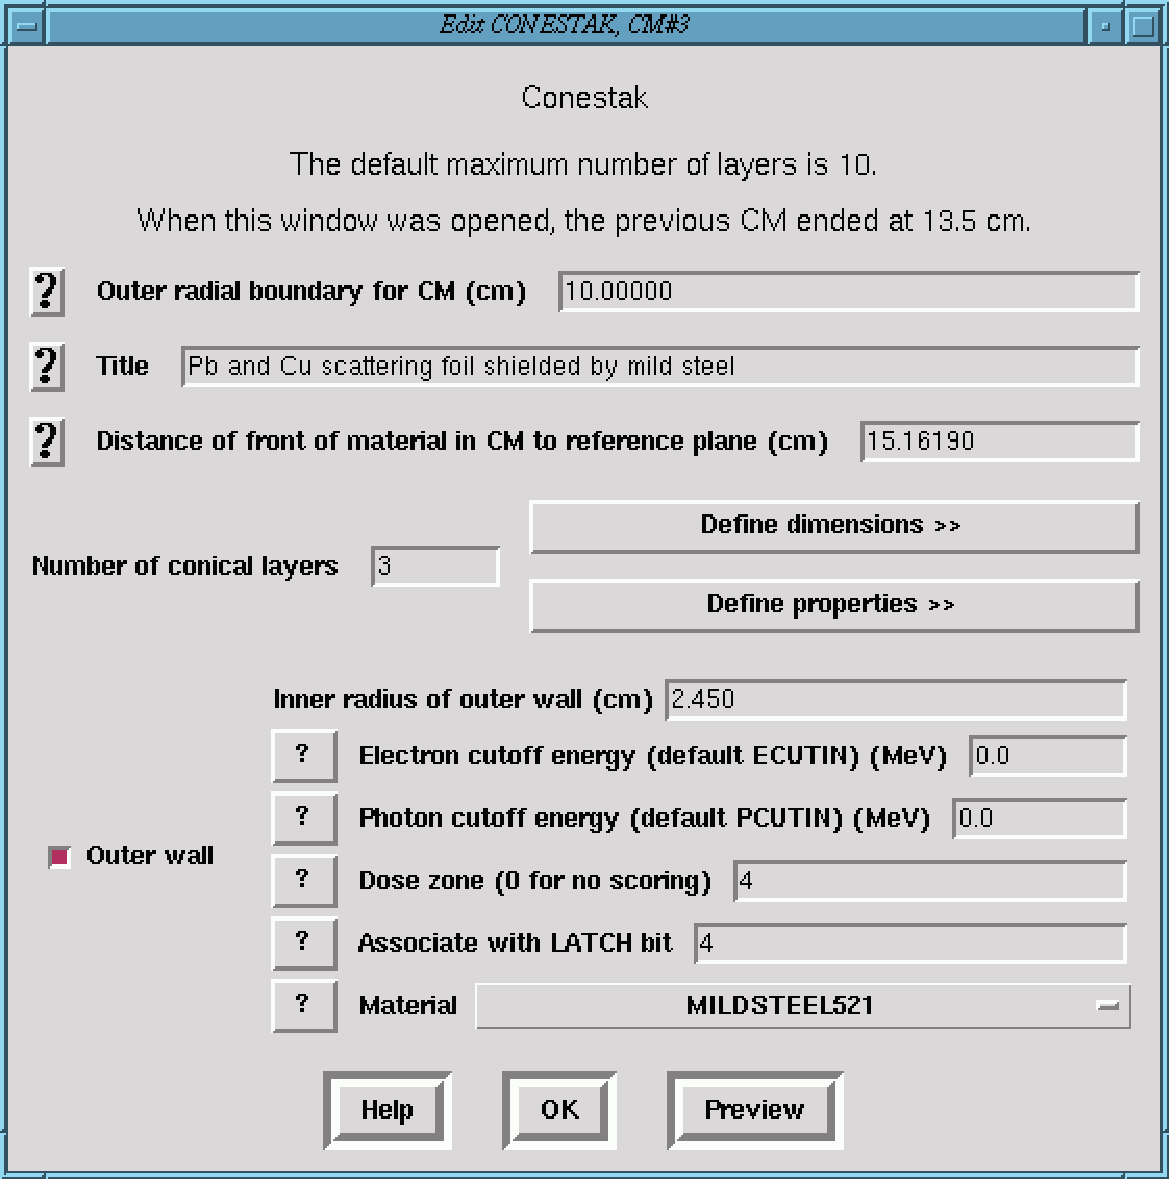
\includegraphics[width=10cm]{figures/conestak}
\end{center}
\caption{A typical CONESTAK CM parameter input window.\label{conestak}}
\end{figure}

\subsubsection{Option to define JAW settings automatically}

The GUI for the JAWS component module allows you to specify the
x/y coordinates of jaw openings in two ways.  You can either input
the coordinates directly, or you can define the coordinates using
field size and SSD.  If you choose the latter option, then a window
will open asking you to specify the half-width, SSD
and the value of Z at the beam focus (usually the front of the photon
target and the point from which the SSD is measured) and
the pairs of jaws that you wish to apply this field to. The Z positions of
the jaws must also be defined.  Once you
have specified these parameters, click on {\sf Update x/y coords.} and
the GUI will calculate the opening coordinates for the selected
jaws and update them
in the ``Define jaws" window.  You can then go on to define different
fields for different pairs of jaws within the same CM.  The algorithm is
based on a simple straight line beam edge and it is only useful for the
settings of the photon beams.  For example, in a 10 cm x10 cm electron beam,
the photon jaws might be set for a 15 x 15 field since the scrapers define
the field size.


\subsection{Previewing components}

The {\sf Preview} button at the bottom of each CM generates a diagram of
the CM based on the parameters you have entered.  (Should an error occur
on previewing a CM, close any new windows and check that
you have entered all parameters.)  Note that you may
need to rescale the axes to show it realistically; this is achieved by
selecting {\sf Change plot properties} on the preview window.  The
default scale maximises the space available in any direction.

One or more canvases may appear, depending on the number of perspectives
required to display the CM geometry.  The mouse cursor position is shown
in the bottom right corner of each canvas.

A separate print button is used for each canvas so that each perspective
may be printed or exported individually.  On selecting {\sf Print}, you will be
prompted to select colour or black and white, portrait or landscape, and
printing to a file or to a printer.

Note that the materials corresponding to the colours used in these
previews  can be seen by selecting {\sf Change colour scheme} in the
{\sf Preview} menu bar.  If a material has not been specified or does not
exist in the PEGS4 file selected, it will be shown as black on the preview.

\subsection{Previewing the accelerator}

The {\sf Preview} menu button on the {\sf BEAMnrc GUI} main window has a
selection {\sf Preview accelerator}, which leads to a 2-dimensional
preview of the entire accelerator.  An option menu located in the lower
left corner of the accelerator preview window allows you to choose
either the x-z cross-section (through y=0) or the y-z cross-section
(through x=0) of the accelerator.

The canvas on which the accelerator
is drawn is contained within scrollbars.  The default scale of the
canvas is 20 pixels per centimetre in the z dimension, and the scale of
the x or y dimension is chosen based on the width of the canvas so that
at least the width of the accelerator is shown without the need for scrolling.
To change the scale, the axis ranges and the number of ticks, select the
{\sf Plot Properties} button.

To print the canvas on which the accelerator is drawn, select the {\sf
Print} button.  Be aware that the diagram will be scaled
automatically to fit on a page; if you want the fonts to be legible it
is recommended that you adjust the zoom factors to scale it properly
before printing.

To the left of the canvas is a legend which shows all of the materials
used in your accelerator and the colours which are used to display
them.  To change any of these colours, click on the colour swatch and
change the RGB values on the sliding scales.  The canvas will be redrawn
using the new colour set.  As with the individual CM previews, if a
material selected is not in the PEGS4 file specified, that material will
appear as black in the preview.

Figure~\ref{preview.example} shows an example of the output of such a
preview.

\begin{figure}[hp]
\begin{center}
\htmlimage{scale=1.0}
\leavevmode
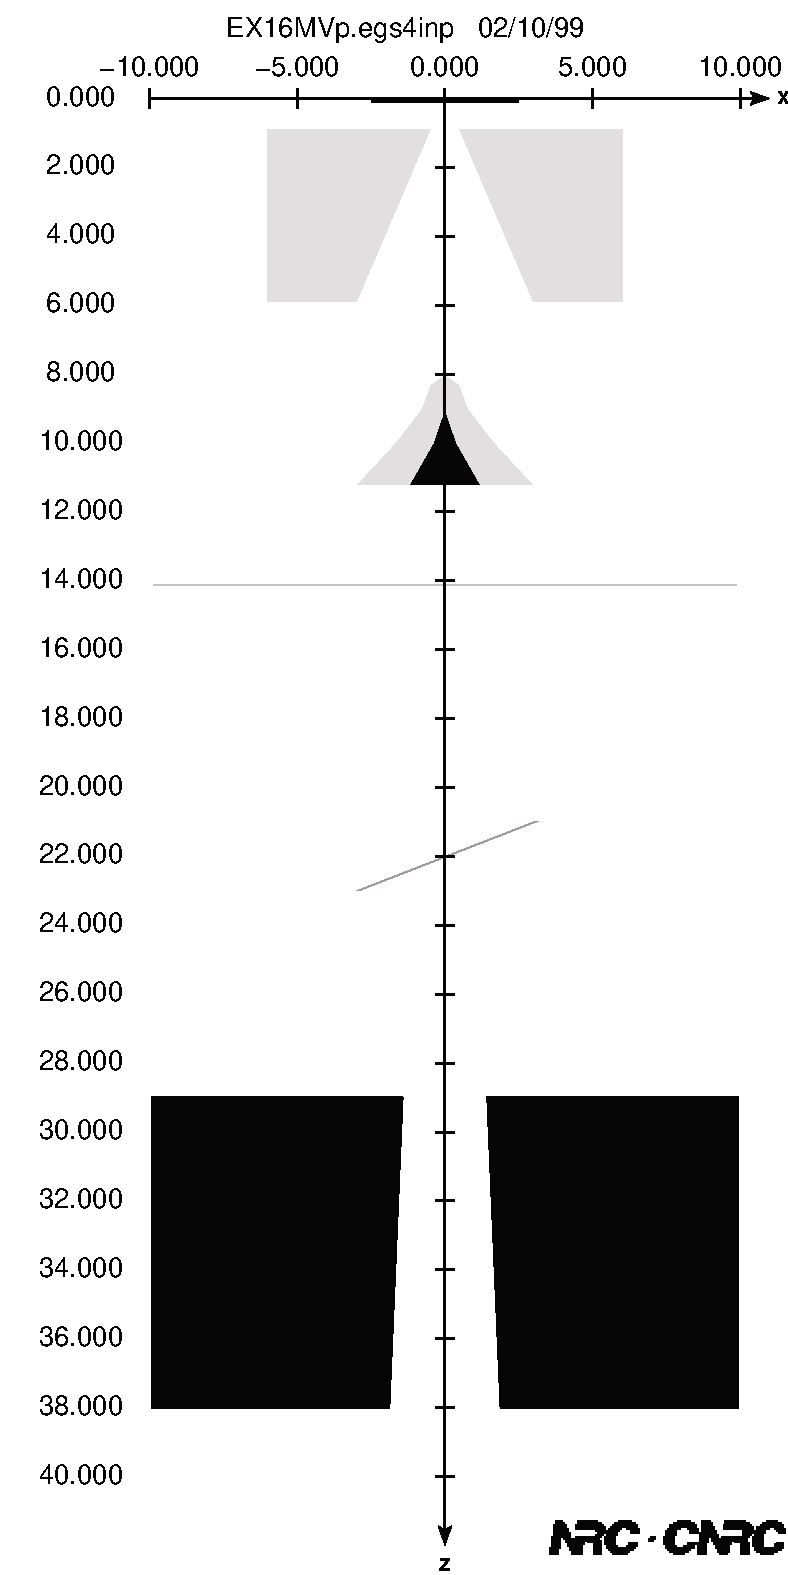
\includegraphics[width=10cm]{figures/EX16MVp_gui}
\end{center}
\caption{Preview of the EX16MVp accelerator example using the ``Preview
accelerator'' option.}
\label{preview.example}
\end{figure}

\subsection{Selecting a colour scheme}

Under the {\sf Preview} menu button on the main {\sf BEAMnrc GUI} window is
the selection {\sf Change colour scheme}.  Selecting this will show a
legend of all the materials available in the PEGS4 cross-sectional data
file and the colours each has been assigned.  To change a colour, click
on the colour swatch and select the new RGB colour to be associated with
that material.

If you prefer to use grey-scale (likely for printing), you can change the
colour scheme to grey-scale by selecting the {\sf Grey-scale}
radio-button.  Then when editing a colour a single scale widget of
intensity is used.

\subsection{Compiling and Running BEAMnrc}

When all of the parameters have been set, select the {\sf Save input file
as...} option from the main window {\sf File} menu.  If the directory
corresponding to the module filename does
not exist, \ie~ {\tt BEAM\_}$<${\em modulename}$>$, you will be asked if
you want to create it before
continuing.  If you don't, the browser will start in your {\tt \$EGS\_HOME}
directory.  Change to the directory that you wish to save the file in,
enter the desired filename and click ``OK'' to write the file.

At this point you may exit the GUI and run the BEAMnrc code from the
command line.  For details on this, see the
BEAMnrc User's Manual\cite{Ro04a}.  You can also run BEAMnrc though the GUI.
Note that for either method {\bfseries you {\it must} save your input file
before starting}.

First you will need to compile the accelerator code.  From the {\sf
Execute} menu, choose {\sf Compile}.  A window with the different
compiler options will appear.  The default options are already set.  If
you would like more information on these options, please see the BEAMnrc
Manual.  Select {\sf COMPILE} to compile the code.  It can take some
time to compile, depending on the speed of your machine and on the size
of your accelerator.  You will be notified when compilation is complete.

Finally, select {\sf Run} from the {\sf Execute} menu.  A window with
the run options appears, defaulting to interactive mode.  If you wish to
submit jobs to a queue, select {\sf batch}. {\sf long} is the default
run time option.  For parallel jobs, select {\sf Run in parallel} and
enter the number of jobs into which to split the run in the text box.
Click {\sf EXECUTE} to execute the code.  You will be notified when the
job is finished.

\subsection{Known bugs and further changes}

There is, unfortunately, no method to make changes to the structure
of an accelerator after it has been made, \ie~ removing a CM, adding a
CM, without rebuilding it entirely.  If you find that you need to do
this, you may have to resort to editing the file manually, or you can build a new
accelerator with the components you want and read in the old file.  The
GUI will encounter an error, but
read the parameters it found before that point.

%%%%%%%%%%%%%%%%%%%%%%%%%%%%%%%%%%%%%%%%%%%%%%%%%%%%%%%%%%%%%%%%%%%%%%%%

\section{The DOSXYZnrc GUI}

To run the DOSXYZnrc GUI from a Linux/Unix window, type {\tt dosxyznrc\_gui}
at the prompt. Note that you must have sourced the Unix script
{\tt egsnrc\_cshrc\_additions} (or {\tt egsnrc\_bashrc\_additions}) in
your {\tt .cshrc} (or {\tt .bashrc}) file.  See the BEAMnrc Manual\cite{Ro04a}
for more information about these scripts.

To run the GUI in a Windows environment, either double click on
the GUI icon or use Windows Explorer to go into directory
{\tt \$OMEGA\_HOME/progs/gui/dosxyznrc} and double click on
{\tt dosxyznrc\_gui}.

DOSXYZnrc requires one input file to be generated by the user, giving a
complete description of the phantom and the source.  At the top level of
the GUI, you are presented with four options:
\begin{enumerate}
\item {\sf Start a new input file}.  This option allows you to start
creating a new set of inputs.  If you select this after having loaded an
input file, those parameters will be discarded.
\item {\sf Load a previous input file}.  This allows you
to select an input file that you have already made.
\item {\sf Edit parameters}.  This takes you to the main editing screen,
whether you
have loaded an input file or not.  On start-up, this option has the same
effect as {\sf Start a new input file}.
\item {\sf Save input parameters as...} allows you to save the input parameters
to a file in your {\tt \$EGS\_HOME/dosxyznrc} directory.

\end{enumerate}

\subsection{Editing DOSXYZnrc parameters}

The {\sf Edit parameters} option takes you to a main window with four
sections.  The first is the title.  It is recommended that you include
the name of the input file in the title as an identifier.  In the second
section, you are asked
to define the phantom for the simulation.  To do this, you can use a
phantom created from CT data, or you can define a phantom
voxel-by-voxel.  Select the radio-button corresponding to the method of
your choice, then click the {\sf Define phantom using...} button.  A new
window will pop up in which you can define the phantom.
The third section of the {\sf Edit parameters} window requires that you
enter general simulation parameters.

\subsection{Loading a previous input file}

The {\sf Load a previous input file} option takes you to a directory
browser from which you can select the input file to load.  The default
filter for the browser is for files with the extension {\tt .egsinp}.
After selecting a file, you will be asked for the name of a PEGS4 data
file.  Note that unlike the BEAMnrc GUI, the DOSXYZnrc GUI does not have the
error-checking routine of testing that the materials listed in the PEGS4
file match those used in the input file.  After selecting the PEGS4
file, the parameter editing window appears.

Similar to the BEAMnrc GUI, the DOSXYZnrc GUI also gives you the option
to specify an existing input file (with accompanying PEGS4 data) as command
line arguments.  From within the {\tt \$EGS\_HOME/dosxyznrc} directory, type:
\begin{verbatim}
dosxyz_gui inputfilename [pegsfilename]
\end{verbatim}
The {\tt .egsinp} and {\tt .pegs4dat} extensions are optional.  If you do not
supply a PEGS4 data file, then a window will immediately open requesting that you
do so.  Note that {\tt inputfilename} must be in the {\tt \$EGS\_HOME/dosxyznrc}
directory.

\subsection{Defining the phantom using CT data}

If you selected phantom definition using CT data, you will be asked to
choose a {\tt .egsphant} file by browsing starting in the current
directory.  These
files can be created using ctcreate.  For more information, please see
section 15 of the 2004 DOSXYZnrc User's manual\cite{WR04a}.

\subsection{Defining the phantom voxel-by-voxel}

With voxel-by-voxel phantom definition, you will be prompted
to choose a {\tt PEGS4} cross-sectional data file (if not already
defined).  This is essential
for defining the materials used in the phantom.  Select the file by
browsing either your {\tt \$EGS\_HOME/pegs4/data} directory or the {\tt
\$HEN\_HOUSE/pegs4/data} area.  If you
select a file from the {\tt \$HEN\_HOUSE/pegs4/data} area which also
exists in your {\tt \$EGS\_HOME/pegs4/data}
directory, you will be asked to select the latter instead.  This is
enforced because DOSXYZnrc, like BEAMnrc, looks first in your {\tt
\$EGS\_HOME/pegs4/data} directory for these files.

Once the {\tt PEGS4} file has been selected, the phantom definition
window will appear, containing 3 sections.  The first step is to define
the voxel dimensions in the x, y and z directions.  To accomplish this,
you have a choice of 2 methods.  You may define the voxels individually
by entering the position of the beginning of each voxel and the end of
each voxel, \eg~for voxel $i$, $x_{i-1}$ and $x_i$ form the
x-boundaries.  You may also define the dimensions in groups by
specifying the number of voxels in the group and the width of each voxel
in the group, for as many groups as is required.

The second step is to define the media used in the phantom.  The number
of media that you intend to use must be entered first, the {\sf
Define media} button selected.  On this new window, an option menu is
used to select each medium.  The first entry,
medium 1, is the default medium.  Once these have been specified, click
on {\sf Define voxel media} to set the medium of individual voxels.  You
only need to explicitly specify the medium of those voxels NOT comprised
of medium 1, the first entry on the previous window.

Finally, set the output option, formerly known as IZSCAN.  Here you may
specify a region for which dose is output.  An x-scan per page means
that each page of output will contain data along the x-axis for one
value of z.  A z-scan
per page means that each page of output will contain data from the
z-direction for one value of y, \eg, if you wanted to see the dose along
the central-axis region.

Four other
parameters are required in this phantom definition section, the global
electron and photon cutoff energies, the maximum step size and an option
which allows you to print a summary of the 20 highest doses.

\subsection{Defining the source}

The next section asks for a definition of the source.  The first option
menu allows you to choose the incident particle type.  Note that ``all''
can only be used when a phase-space source is selected.  The source
available include standard source types and phase space sources which
may be obtained from
the output of BEAMnrc.  Figure~\ref{xyz_source} shows the window for
defining source options for a parallel beam from the front.
Radio-buttons allow the user to choose between a monoenergetic beam or
spectrum.  The {\sf Help} button generates a window with a
complete description of the parameters required for each source.

\begin{figure}[htb]
\begin{center}
\htmlimage{scale=2.0}
\leavevmode
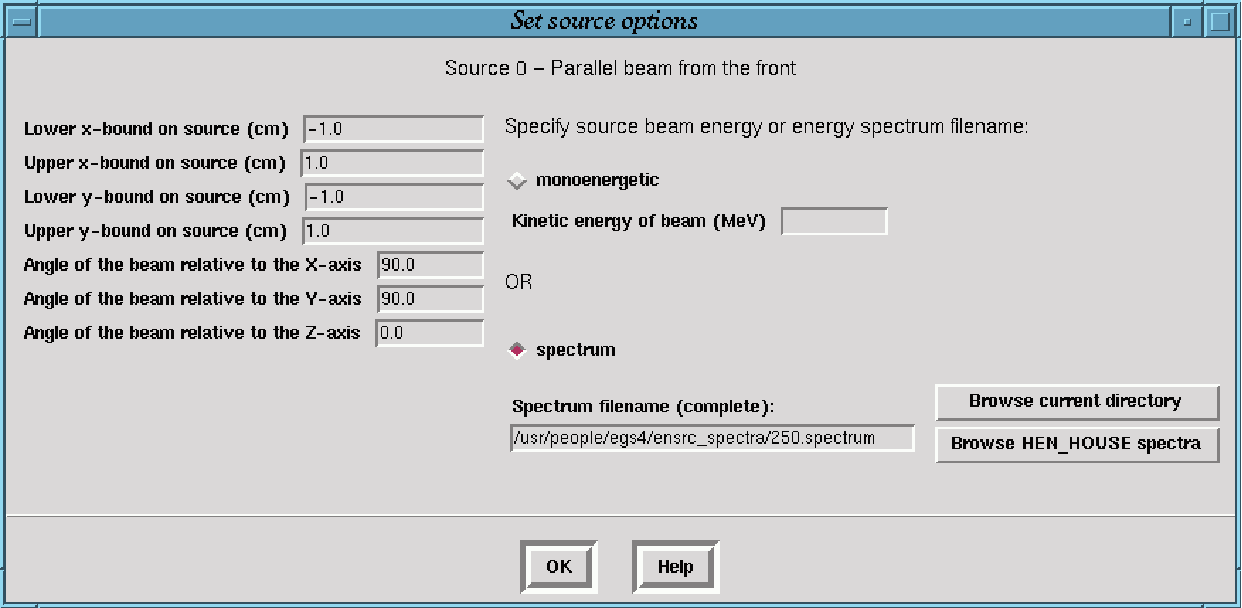
\includegraphics[width=15cm]{figures/xyz_source}
\end{center}
\caption{The source option window for a parallel beam from the front.\label{xyz_source}}
\end{figure}

For phase space sources, in addition to the parameters required for the
source, the thickness and medium of the region surrounding the phantom
should be input.  The default medium is VACUUM and the default thickness
is 50cm.  The phase space beam input file should be selected by browsing
your home directory or {\tt \$OMEGA\_HOME}.  The format of this file
must also be specified.  You may also choose to use inclusive and/or
exclusive bit filters to calculate the dose.  To do so, select the
{\sf Phase space input + dose components} radio-button.  The option menu
for bit filters will then become active and you may set the type of
filter and the bits to include/exclude.

\subsection{Simulation parameters}

The third section of the {\sf Edit parameters} window requires that you
enter general simulation parameters, such as the number of histories,
IWATCH output, maximum CPU time, random number generator seeds,
incident beam size, phase space
redistribution, run option, output restart data, range rejection and ESAVE
inputs.  The help buttons to the left of each parameter will
provide you with the information necessary to properly specify these
values.

\subsection{EGSnrc parameters}

Similar to the BEAMnrc GUI, the DOSXYZnrc GUI allows you to edit the
EGSnrc input parameters.  This is done by clicking on the
{\sf Edit EGSnrc Parameters} button at the bottom of the
{\sf Edit parameters} window.  This will open up a window identical
to that used to set EGSnrc parameters in the BEAMnrc GUI.
If you are working
from an EGS4/DOSXYZ file or starting from scratch, the EGSnrc parameters
will be set to their defaults.  When you save the file,
these parameters will be appended to the end of the {\tt .egsinp} file
in a specific text-based format.  See the DOSXYZnrc manual for a more
detailed description of the EGSnrc input parameters.

\subsection{Compiling and running DOSXYZnrc}

Once the parameters have been completely defined, select
{\sf Save and close} on the {\tt Edit parameters} window or
{\sf Save input parameters as...} on
the main {\sf File} menu.  The browser will start in the
directory that you are running the GUI from.  Enter a filename and click
``OK'' to save the file.

At this point you may exit the GUI and run DOSXYZnrc from the command line,
or use the
GUI as a front end by selecting {\sf Compile} the {\sf Run} from the
{\sf Run} menu.  Please
refer to the DOSXYZnrc User's Manual\cite{WR04a} for more details on how to run dosxyznrc
from the command line, and for details on the various compiling and
execution options.

%%%%%%%%%%%%%%%%%%%%%%%%%%%%%%%%%%%%%%%%%%%%%%%%%%%%%%%%%%%%%%%%%%%

\section{The BEAMDP GUI}

The BEAMDP GUI greatly facilitates running BEAMDP by not requiring
the user to re-enter parameters from scratch every time phase space
data is analyzed.

In a Linux/Unix window, the GUI is invoked by typing {\tt beamdp\_gui}.
Note that you must have sourced the Unix script
{\tt egsnrc\_cshrc\_additions} (or {\tt egsnrc\_bashrc\_additions}) in
your {\tt .cshrc} (or {\tt .bashrc}) file.  See the BEAMnrc Manual\cite{Ro04a}
for more information about these scripts.

To run the GUI in a Windows environment, either double click on
the GUI icon or use Windows Explorer to go into directory
{\tt \$OMEGA\_HOME/progs/gui/beamdp} and double click on
{\tt beamdp\_gui}.

The {\sf Help} menu option will show you a list of the available
options on the main menu and their meanings.
There is on-line help for any option which is not self-explanatory;
simply press the ``?'' to the left of the option.
Please refer to the BEAMDP User's Manuals\cite{MR04a,MR04b}
for further information.

To get multiple graphs on the same plot, simply make any changes to the
data and execute again.  If the file exists, the GUI will prompt you for
whether you want to add this graph or overwrite the file with it.  If
you want multiple plots, select {\sf Add}.

\section{References}

\bibliography{../irs}
\bibliographystyle{unsrt}

\end{document}
